\begin{figure*}[t]
    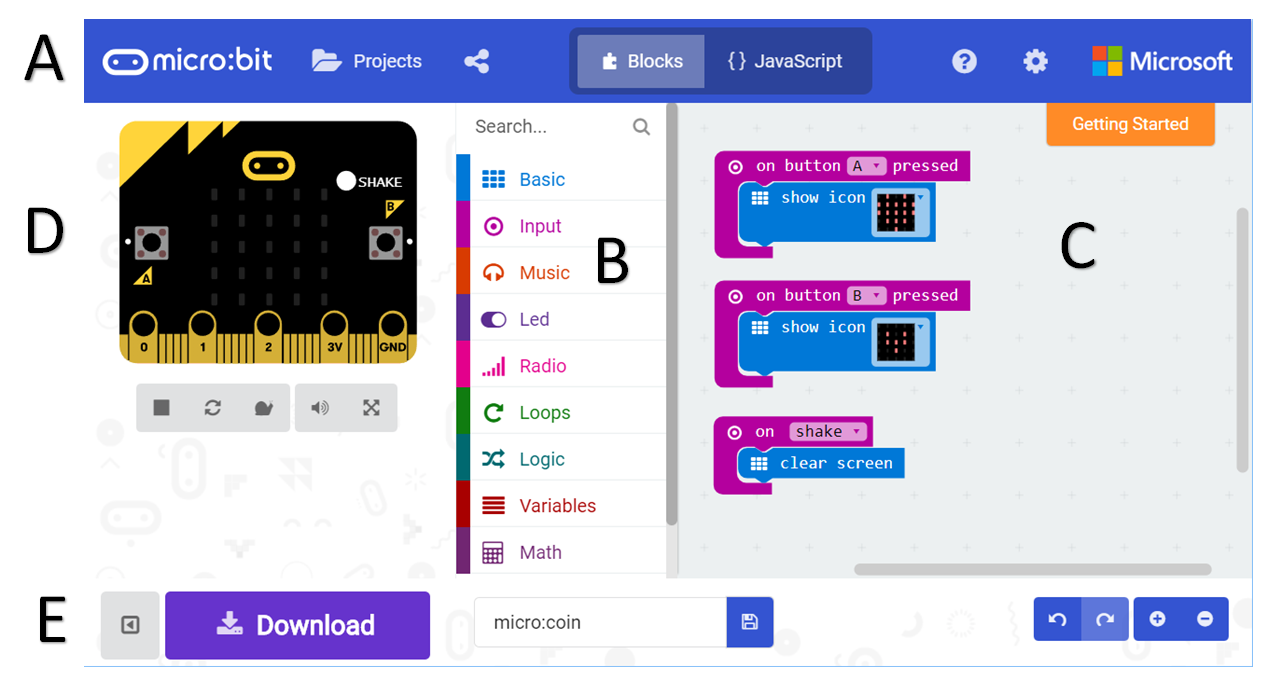
\includegraphics[width=6in]{images/webApp.png}
    \caption{\label{fig:snapshot}MakeCode web app for the micro:bit (\url{http://makecode.microbit.org}).}
  \end{figure*}

\section{The BBC micro:bit}

% Talk about the motivations, make people care, provide concrete deliverables

As mentioned in the Introduction, the motivation for the BBC micro:bit project
stemmed from the BBC's previous history with computing education and the BBC Micro
project, the desire to address the growing digital divide in the UK~\cite{XYZ}, 
as well as the UK government's mandate to each computer science at the K-12 grade levels. 

The goals for the BBC micro:bit project were:
\begin{itemize}
    \item[B1] to provide a simple creative experience for physical computing, wearable and Internet of Things (IoT) projects;
    \item[B2] to supply a device that can continue to provide learning opportunities as the user's expertise grows.
    \item[B3] to give students an exciting, engaging introduction to coding;
    \item[B4] to stimulate curiosity about how computing technologies can be utilized to solve problems that students identify.
\end{itemize}

{\bf [BBC prototype by Michael Sparks and user trials] }

In December 2014, the BBC issued an Request for Participation
for ``Delivery of a hands-on learning experience for the Make it Digital season'',
which was the micro:bit project.
Twenty-nine partners were invited to contribute hardware, software, services,
teaching materials, packing/distribution, logistics, events and funding.
Work on the project commenced in February 2015, with delivery of
a web site/app in September 2015 (which was critical
for training teachers) and delivery of the micro:bits in the second
half of the 2015-2016 school year.

\subsection{Why physical computing?}

Really need Howard Baker's input on this.

\begin{itemize}
    \item broad reach
    \item topical
\end{itemize}

\subsection{The hardware}

Figure~\ref{fig:microbit} shows (a) the front and (b) the back of the
micro:bit, which measures 4cm x 5cm. The aesthetic of the micro:bit is designed to be engaging from the off, with streaks of hair (upper left) and a friendly face (upper middle).
The micro:bit board hosts a variety of sensors (temperature, accelerometer, magnetometer,
light level), a 5x5 LED matrix, two user-defined buttons, as well as Bluetooth
Low Energy (BLE) communications.\footnote{The micro:bit has a whopping
16kB of RAM and 256kB of Flash memory, compared to the Uno's 2kB of
RAM and 32kB of Flash}. More importantly, the device embraces these sensors in its design bringing them to the fore, so to expose its users to the future: a world of embedded, Internet enabled devices.

In contrast to the Uno which has no built-in sensors, the micro:bit
allows many projects to be completed with no additional hardware or wiring.
The holes on micro:bit's edge connector allows additional external sensors and actuators to be connected via crocodile clips or banana plugs.
The micro:bit's BLE capabilities introduces networking to the
picture, and enables streaming of data and command/control operations among the micro:bit,
smartphones, laptops, as well as other micro:bits.
As with Arduino, an ecosystem of micro:bit shields
(hardware peripherals) that accommodate the micro:bit's edge
connector expands its capabilities (\url{http://microbit.org/resellers/}).

%% floating sentence, should be optimised some how -- is there a bit that talks about programming?
The micro:bit can be programmed over USB via a host computer (usually a laptop or desktop)
and then embedded in projects where it runs on battery power.

The unique combination of features supplied by the micro:bit enables a creative, extensive experience for physical computing (B1, B2).

\subsection{The software}

The design of the micro:bit coding tools also was oriented towards a
simple starting experience with room for progression (B3, B4). Based on in-school trials with a micro:bit prototype, the BBC focused on delivering a web app
based on the popular Blockly framework~\cite{Blocky2015} to permit students to
create scripts via drag-and-drop operations in a web browser, and see
the execution of their scripts via a simulator; text-based coding via scripting languages also
was identified as an important feature. As the micro:bit would be incorporated
into standalone projects, it also was essential for the user's program to be stored on the device for future untethered execution via battery power.

%final design put the entire toolchain in web app, without need to invoke C/C++ compiler to
%compile the user's program; ARM DAPlink solution makes micro:bit appear as USB pen drive
%on all operating systems; MicroPython provided second programming solution with entire toolchain
%on the micro:bit!!]

% less techy here

The solution delivered by the BBC's partners evolved from the initial
design to include support for Blockly, JavaScript and Python, all
via web apps.
Figure~\ref{fig:snapshot} shows a screen snapshot of the MakeCode web app
for the micro:bit,
which supports programming via both Blocky and JavaScript.
The web app has five main sections: (A) menu bar with access to projects
and examples, and switching between Blockly and JavaScript editors; (B)
Blockly toolbox of micro:bit API categories; (C) Blockly programming
canvas with a simple reactive program; (D) micro:bit simulator for execution
of the user's program in browser; (E) download button, which invokes the in-browser
compiler/linker to produce a binary executable.

% The event-based program shown in section (C) displays a large heart when the
% A button is pressed, displays a small heart when button B is pressed,
% and clears the display when the user shakes the micro:bit (shake
% detection is implemented using the accelerometer; in the simulator, the
% shake event is fired using a virtual button). In addition to event-based
% APIs, direct access to the micro:bit's sensors via polling is possible.

The Python solution for the micro:bit is based on MicroPython (\url{http://micropython.org})
an implementation of Python 3.0 for microcontrollers. It includes
a full Python compiler and runtime that runs on the micro:bit and
supports a read-eval-print loop (REPL) to execute commands sent via
a terminal, as well as to import and run scripts from the Python web app for
the micro:bit (\url{http://python.microbit.org}).

% \begin{itemize}
% \item
% \item an efficient C++ runtime for the micro:bit created by Lancaster
% University;
% \item a web app
% with Blockly and JavaScript editors, micro:bit simulator,
% and a compiler to machine code (linked against a pre-compiled
% C++ runtime image, so no C++ compiler is needed for user code);
% \item a Python compiler and read-eval-print loop (REPL) that resides
% {\em on the micro:bit} (via \url{https://micropython.org/}),
% supported by a simple web app (\url{http://python.microbit.org}) and
% an installable application (\url{https://codewith.mu/});
% \item ARM's DAPlink firmware makes the micro:bit appear as USB pen drive
% on most operating systems, enabling a simple file copy operation to
% install a user's program on the micro:bit (no device drivers needed).
% \end{itemize}
% MakeCode, MicroPython, and the C++ runtime are all open source.\footnote{
% At \url{https://github.com/microsoft/pxt},
% \url{https://github.com/micropython/micropython},
% and \url{https://github.com/lancaster-university/microbit-dal},
% respectively.}


% \subsection{Content and training}

% The BBC micro:bit project also called for partners to develop content
% and to ``train the trainers'' (educators) around the micro:bit computing
% system.  This built on efforts by the non-profit Computing At Schools
% (\url{www.cas.org}) organization to train UK educators to teach computer
% science.

%- A lot of lessons learned from delivering end-to-end experience in UK and other countries
%   - hardware (unique design, as already mentioned)
%   - firmware:  high-level C/C++ runtime and ARM's DAPlink
%   - web-based IDE: no C/C++ compiler needed to compile user code
%   - content
%   - training
% In country partnerships

% main points
% - mass participation
% - country readiness (or perhaps willingness)

% :@ no overviews xx James
% \subsection{Overview}

% Section~\ref{sec:physical} reviews physical computing, which anchors
% and defines the micro:bit experience. Section~\ref{sec:projects}
% presents a broad set of micro:bit-based projects, ranging
% from wearable games to environment science, that demonstrate
% the micro:bit's capabilities.  Section~\ref{sec:country}
% describes the rollout of the micro:bit in the UK and other countries
% in Europe, the Americas and Asia. Section~\ref{sec:conclude}
% concludes with final thoughts about what has made the micro:bit
% successful to date and what comes next.


% compared to Arduino
% https://twitter.com/adamwwolf/status/1019070808038072320

% success of micro:bit due to
% - Low-cost, simplicity
% - Partnerships (hardware, software, content, training)
% - Open Source of software (CODAL, MakeCode, ...)
% - Hardware Reference design

% - why is it interesting?
%   - edge/physical/IoT computing
%   - build off of Scratch/Blockly, but untethered (via in-browser compiler)
%   - transition to JavaScript and Python

% - BBC rollout in UK
% - Global reach
%    - BBC rollout mirrored in other countries
%    - Communities
%      - Sri Lanka user group: http://microbitslug.org/
%      - UK libraries (loan program)
%    - third party editors









